%%
%% ****** ljmsamp.tex 13.06.2018 ******
%%
\documentclass[
11pt,%
tightenlines,%
twoside,%
onecolumn,%
nofloats,%
nobibnotes,%
nofootinbib,%
superscriptaddress,%
noshowpacs,%
centertags]%
{revtex4}
\usepackage{ljm}
\usepackage{listings}

\lstset{
language=C++,
basewidth=0.5em,
xleftmargin=45pt,
xrightmargin=45pt,
basicstyle=\small\ttfamily,
keywordstyle=\bfseries\underbar,
numbers=left,
numberstyle=\tiny,
stepnumber=1,
numbersep=10pt,
showspaces=false,
showstringspaces=false,
showtabs=false,
frame=trBL,
tabsize=2,
captionpos=t,
breaklines=true,
breakatwhitespace=false,
escapeinside={\%*}{*)}
}

\begin{document}

\titlerunning{RANS/ILES method optimization} % for running heads
\authorrunning{L.~A.~Benderskiy, D.~A.~Lyubimov, A.~A.~Rybakov} % for running heads

\title{RANS/ILES Method Optimization\\
for Effective Calculations on Supercomuter}
% Splitting into lines is performed by the command \\
% The title is written in accordance with the rules of capitalization.

\author{\firstname{L.~A.}~\surname{Benderskiy}}
\email[E-mail: ]{leosun.ben@gmail.com}
\affiliation{Joint Supercomputer Center of the Russian Academy of Sciences - branch of Scientific Research Institute of System Analysis of the Russian Academy of Sciences, Leninsky prospect 32a, Moscow, 119334, Russia}

\author{\firstname{D.~A.}~\surname{Lyubimov}}
\email[E-mail: ]{dalyubimov@ya.ru}
\affiliation{Joint Supercomputer Center of the Russian Academy of Sciences - branch of Scientific Research Institute of System Analysis of the Russian Academy of Sciences, Leninsky prospect 32a, Moscow, 119334, Russia}

\author{\firstname{A.~A.}~\surname{Rybakov}}
\email[E-mail: ]{rybakov.aax@gmail.com}
\affiliation{Joint Supercomputer Center of the Russian Academy of Sciences - branch of Scientific Research Institute of System Analysis of the Russian Academy of Sciences, Leninsky prospect 32a, Moscow, 119334, Russia}


\firstcollaboration{(Submitted by S.~S.~Submitter)} % Add if you know submitter.
%\lastcollaboration{ }

\received{June 13, 2018} % The date of receipt to the editor, i.e. December 06, 2017

\begin{abstract}
TODO
\end{abstract}

\subclass{68N19} % Enter 2010 Mathematics Subject Classification.

\keywords{TODO.} % Include keywords separeted by comma.

\maketitle

% Text of article starts here.

\section{Introduction}

TODO

\section{Section 1}

TODO

\section{Section 2}

TODO

\section{Realization of linked border conditions}

The RANS / ILES method works with block-structured grids, which consist of separate blocks interconnected by interfaces.
Each block of the computational grid is an ordered three-dimensional array of cells, which can be accessed by indices.
This greatly simplifies the work with the grid within one block.
Associated with each cell is a set of gas-dynamic parameters.
Each block of the computational grid has its own three-dimensional curvilinear coordinate system, the axes of which are directed along the edges of the block.
Interfaces describing the contact of blocks with each other contain information about the coordinates of the touch of sections of both blocks (in terms of nodes of the computational grid), as well as information about the coordination of coordinate systems of the related blocks.
Some faces of the grid blocks do not touch other blocks, but are the boundary of the computational domain.
In this case, it is necessary to describe the boundary conditions.
This is done with the help of special objects that describe the boundary conditions on a given rectangular section of the block boundary.

When carrying out calculations, calculation grids consisting of identical sectors are often used.
That is, in essence, such a grid is a grid with a smaller number of cells, duplicated several times and rotated relative to the original one around a given straight line.
To obtain a solution to the gas-dynamic problem, it is sufficient to perform calculations for only one such sector.
However, during the calculations it is necessary to observe additional conditions.
When calculating a separate sector, it is necessary to take into account that the output flows at the individual block boundaries must coincide with the input flows at the boundaries of other blocks, and these boundaries are spaced apart.
Such boundary conditions will be called bound.
To increase the efficiency of the account using the RANS / ILES method, this type of boundary conditions was implemented.

One of the main operations performed on the associated boundary conditions is to determine whether they correspond to each other.
With automatic marking of the associated boundary conditions of the selected sector of the computational grid, a compliance check is performed, with which pairs of the associated boundary conditions are found.
Two types of search for connections between boundary conditions are implemented: boundary conditions combined by parallel transfer and rotation around a given axis.
To determine whether the two boundary conditions are consistent with each other, you need to combine them with the help of a given type of movement so that their centers coincide, and then check whether their corner nodes coincide (Fig.~\ref{fig:match3}).

\begin{figure}[h]
\setcaptionmargin{5mm}
\onelinecaptionsfalse
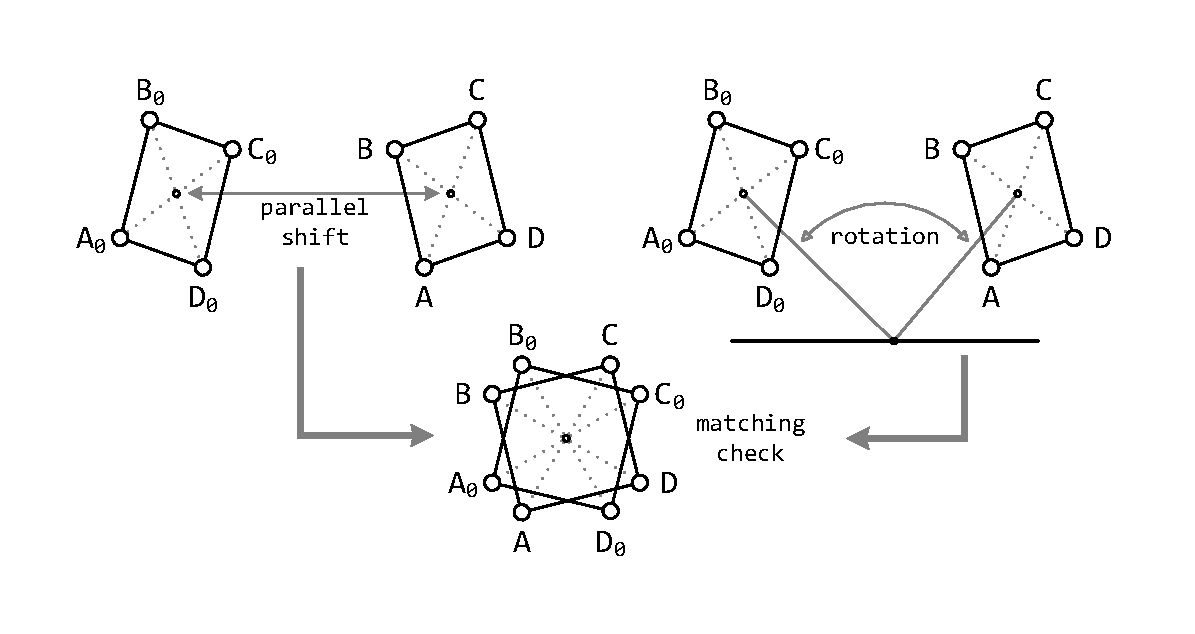
\includegraphics[width=0.95\textwidth]{pics/match3.pdf}
\captionstyle{normal}
\caption{Connection of linked border conditions to each other \\ using parallel shift and rotation around a straight line.}
\label{fig:match3}
\end{figure}

Checking the coincidence of the corner nodes of two potentially related boundary conditions is determined by considering four possible cases, taking into account the renaming of vertices: the figure $A_0B_0C_0D_0$ can coincide with one of the figures $ABCD$, $DABC$, $CDAB$, $BCDA$ (Fig.~\ref{fig:match}).

\begin{figure}[h]
\setcaptionmargin{5mm}
\onelinecaptionstrue
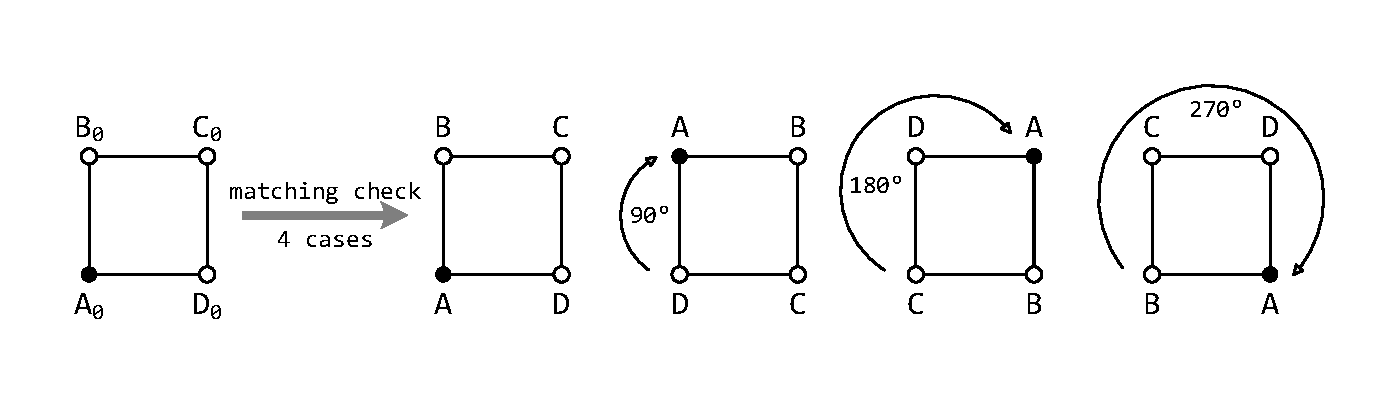
\includegraphics[width=0.95\textwidth]{pics/match.pdf}
\captionstyle{normal}\caption{Four cases for checking the coincidence of the corner points of the border conditions.}
\label{fig:match}
\end{figure}

The order of checking the correspondence of the corner nodes $A_0B_0C_0D_0$ and $ABCD$ of the two boundary conditions is presented in Fig.~\ref{fig:match2}.
In addition to the fact that the angular nodes of a pair of boundary conditions coincide, a correspondence between their coordinate systems is also established.
This allows for any cell of a single boundary condition to find the corresponding cell from the associated boundary condition.
All further transformations of the associated boundary conditions (renaming, splitting the boundary condition or parent blocks) are performed only simultaneously.

\begin{figure}[h]
\setcaptionmargin{5mm}
\onelinecaptionstrue
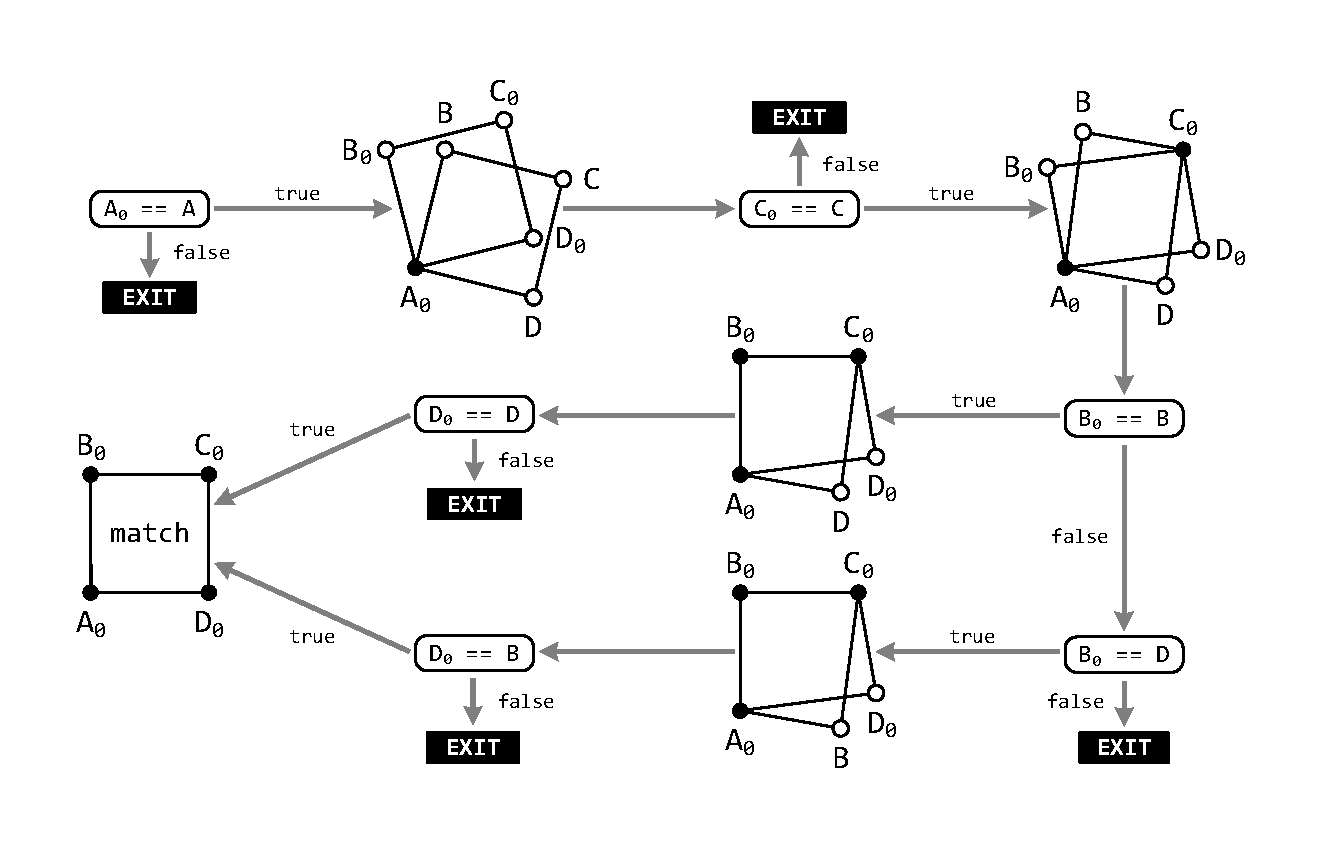
\includegraphics[width=0.95\textwidth]{pics/match2.pdf}
\captionstyle{normal}\caption{Checking the coincidence of the corner points of the border conditions.}
\label{fig:match2}
\end{figure}

\section{Scalability of calculations investigation \protect\\ when cutting the computational grid}

In this section, we describe the experimental launches and analyze the scalability results obtained using the mechanisms of coupled boundary conditions and fragmentation of the computational grid.

For testing, we used a computational grid describing the combustion chamber and containing 94,3 million cells (we will call it a complete grid).
The mechanism of coupled boundary conditions allowed us to replace the calculations on this large grid with calculations made on a sector representing the $1/10$ part of the original grid (36 degrees relative to the $OX$ axis).
The computational grid describing one sector contains 10,7 million cells, which is 9 times smaller than the initial grid.
At the same time, the calculation time is also reduced by 9 times.

The experiments were performed on a segment of the MVS-10P supercomputer located at the JSCC RAS.
This segment consists of computing nodes based on Intel Xeon Phi Knights Landing 7290 microprocessors.
From 1 to 32 computing nodes were used for launches.

First, calculations were carried out on a full grid.
This grid contains 300 calculation blocks, calculations on it are scaled to 32 nodes linearly (the execution time of calculations at 32 nodes is less than the calculation time on one node by almost 32 times).

The computational grid describing one sector contains only 30 nodes, so the calculations on it are much worse scaled.
To analyze the scalability, crushing of this grid was performed by dividing the largest block in half.
In this algorithm, at each iteration, a block is selected that contains the largest number of cells and is divided in half.
The algorithm finishes its work when the resulting blocks can be distributed between the specified number of processes in such a way that the maximum deviation from the average value does not exceed the specified threshold.
The Table~\ref{tab:grids} shows examples of crushing, for which calculations were subsequently made.

\begin{table}[!h]
\setcaptionmargin{0mm}
\onelinecaptionsfalse
\captionstyle{flushleft}
\caption{Characteristics of computational grids.}
\bigskip
\begin{tabular}{|c|c|c|c|c|}
\hline
grid description & blocks/scopes & interfaces & border conditions & linked border cond. \\
\hline
360 deg. (94.3 mln cells) & 300 & 1 796 & 1 643 & 0 \\
36 deg. (10.7 mln cells) & 30 & 152 & 204 & 14 \\
\hline
36 deg., cut for 16 proc. (10\% dev.) & 39 & 224 & 218 & 14 \\
36 deg., cut for 32 proc. (10\% dev.) & 54 & 340 & 248 & 14 \\
36 deg., cut for 64 proc. (10\% dev.) & 170 & 982 & 429 & 23 \\
\hline
36 deg., cut for 64 proc. (1\% dev.) & 383 & 2 356 & 682 & 34 \\
\hline
\end{tabular}
\label{tab:grids}
\end{table}

In Fig.~\ref{fig:g_36_2} graphs of adjacency of blocks of computational grids obtained as a result of crushing are presented.
The nodes of the adjacency graph of the computational grid blocks are the centers of the design blocks.
Two nodes of the graph are connected by an edge if the two corresponding blocks are adjacent.

\begin{figure}[h]
\setcaptionmargin{5mm}
\onelinecaptionsfalse
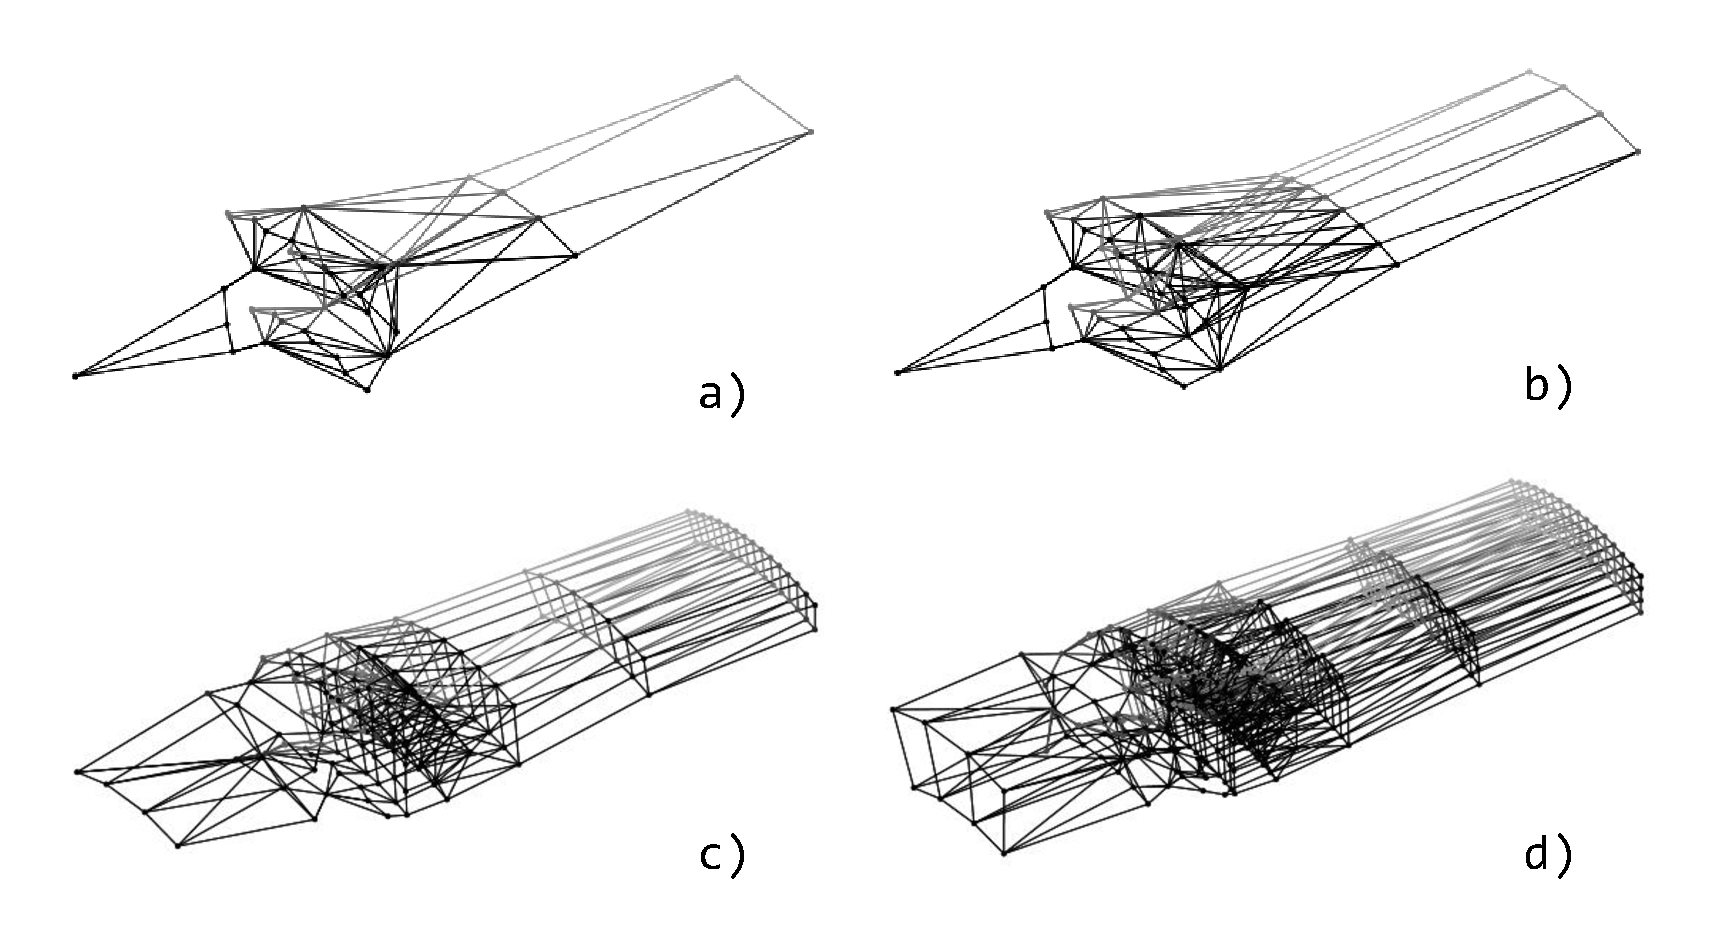
\includegraphics[width=0.95\textwidth]{pics/g_36_2.pdf}
\captionstyle{normal}\caption{Borders adjacency graphs for different cases of computational grid cutting: \\ a - cutting for 16 processes (10\% deviation), b - cutting for 32 processes (10\% deviation), \\ c - cutting for 64 processes (10\% deviaton), d - cutting for 64 processes (1\% deviation).}
\label{fig:g_36_2}
\end{figure}

Fig.~\ref{fig:plot_36_scaling_2} shows the data of calculation runs performed on the same sector (small grid) with various parameters of the grid refinement.
It can be seen that the acceleration of calculations on the initial grid reaches approximately 4-5, and then all the dependencies on the number of nodes used do not change.
This indicates that there is a large block in the grid, so the processing speed of the entire grid is limited from below by the processing speed of this block by one process.
When grinding the grid for distribution by 16 processes (with a maximum deviation of 10\%), the scaling of the calculations improves, but with an increase in the number of computing nodes to 16 or more, the same effect is observed.
When grinding the grid for distribution to 32 or 64 processes (with a maximum deviation of 10\%), the results of scaling are much better.
The dependence of the acceleration on the number of nodes used becomes almost linear, although with a large number of computational nodes, some fluctuations are observed.

\begin{figure}[h]
\setcaptionmargin{5mm}
\onelinecaptionstrue
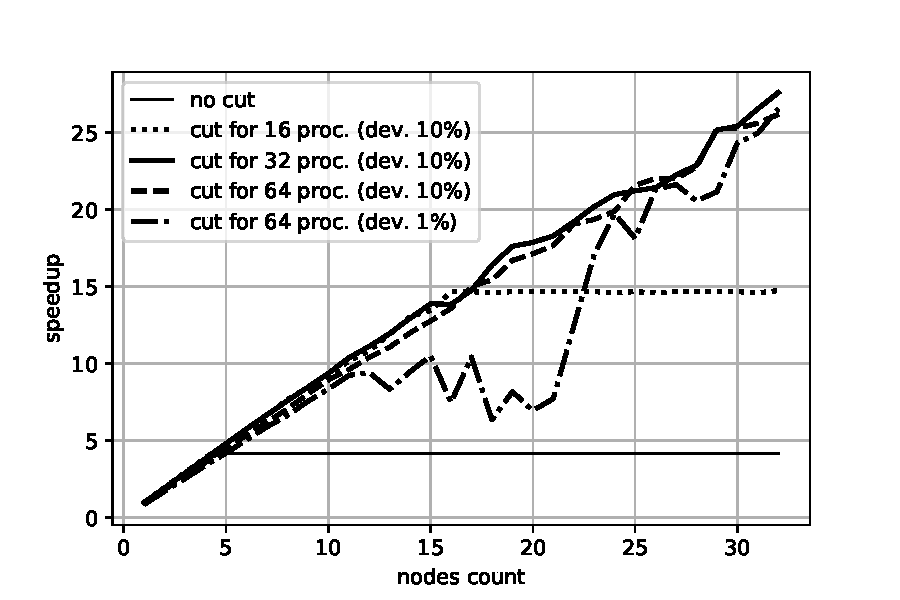
\includegraphics[width=0.95\textwidth]{pics/plot_36_scaling_2.pdf}
\captionstyle{normal}\caption{Graph scaling calculations when using different options for cutting the grid.}
\label{fig:plot_36_scaling_2}
\end{figure}

Also in Fig.~\ref{fig:plot_36_scaling_2} the data of the launches performed on the grid, which is fragmented very finely.
The grid was crushed for distribution to 64 processes, while the maximum allowable deviation from the average computational load was taken as 1%.
The graph shows a very serious drawdown of scaling in the range from 10 to 20 computing nodes.
This is due to the fact that unnecessarily fine crushing leads to the appearance of a huge number of computational blocks and inter-processes between them.
In some cases, blocks can be distributed so inter-computing processes that the amount of data involved in inter-process exchanges between them, becomes critical.
In such situations it is necessary to take into account the factor of interprocess exchanges or not to resort to excessive fragmentation of the grid.

\section{Conclusion}

The results of practical experiments have shown that the mechanisms for preparing the block-structured computational grid for the RANS / ILES method help to achieve multiple acceleration of calculations when performing calculations on a supercomputer.
In particular, the calculations on the grid considered in the article, containing 94,3 million cells, were replaced by calculations on a smaller grid using the mechanism of coupled boundary conditions.
This fine grid was fragmented to achieve linear scaling when running on 32 nodes of the supercomputer.
The total decrease in the counting rate achieved using the two mechanisms described above exceeded 2 orders of magnitude when using 32 compute nodes.

\begin{acknowledgments}
The work has been done at the JSCC RAS as part of the state assignment for the topic 0065-2018-0409 <<Development of architectures, system solutions and methods for creating computing systems and distributed environments of the multi-petaflops performance range, including non-traditional microprocessor architectures>>. The supercomputer MVS-10P, located at the JSCC RAS, was used for calculations during the research.
\end{acknowledgments}

\begin{thebibliography}{99}

\bibitem{Krappel}
\refitem{article}
T.~Krappel, S.~Riedelbauch, \textquotedblleft Scale Resolving Flow Simulations of a Francis Turbine Using Highly Parallel CFD Simulations\textquotedblright, W.~E.~Nagel et al. (Eds.): High Performance Computing in Science and Engineering'16, pp.~499--510 (2016).

\bibitem{Rybakov}
\refitem{article}
A.~A.~Rybakov, \textquotedblleft Inner Respresentation and Crossprocess Exchange Mechanism for Block-Structured Grid for Supercomputer Calculations\textquotedblright, Program systems: Theory and Application, No.~8:1(32), pp.~121--134 (2017) [In Russian].

\bibitem{Jeffers_KNL}
\refitem{book}
J.~Jeffers, J.~Reinders, A.~Sodani, \emph{Intel Xeon Phi Processor High Performance Programming, Knights Landing Edition}, (Morgan Kaufmann, 2016).

\bibitem{Lyub_RANS_ILES}
\refitem{article}
D.~A.~Lyubimov, \textquotedblleft Development and Application of a High-Resolution Technique for Jet Flow Computation Using Large Eddy Simulation \textquotedblright, High Temperature, Vol.~50, No.~\textbf{3}, pp.~420--436 (2012).

\bibitem{Ben_Lyub_Chest_RANS_ILES}
\refitem{article}
L.~A.~Benderskii, D.~A.~Lyubimov, A.~O.~Chestnykh, B.~M.~Shabanov and A.~A.~Rybakov, \textquotedblleft The Use of the RANS/ILES Method to Study the Influence of Coflow Wind on the Flow in a Hot, Nonisobaric, Supersonic Airdrome Jet during Its Interaction with the Jet Blast Deflector \textquotedblright, High Temperature, Vol.~56, No.~\textbf{2}, pp.~247--254 (2018).

\bibitem{Blazek}
\refitem{book}
J.~Blazek, \emph{Computational Fluid Dynamics: Principles and Applications}, (Elsevier, 2001).

\bibitem{Farrashkhalvat}
\refitem{book}
M.~Farrashkhalvat, J.~P.~Miles, \emph{Basic Structured Grid Generation, With an Introduction to Unstructured Grid Generation}, (Butterworth-Heinemann, 2003).

\bibitem{Liseikin}
\refitem{book}
V.~Liseikin, \emph{Grid Generation Methods}, (Springer, 2010).

\bibitem{Queen}
\refitem{book}
M.~Queen, \emph{Parallel Programming in C with MPI and OpenMP}, (Mc-Grow Hill, 2004).

\end{thebibliography}

\end{document}
